\documentclass[10pt,twocolumn,letterpaper]{article}

\usepackage{cvpr}
\usepackage{times}
\usepackage{epsfig}
\usepackage{graphicx}
\usepackage{amsmath}
\usepackage{amssymb}

% Include other packages here, before hyperref.

% If you comment hyperref and then uncomment it, you should delete
% egpaper.aux before re-running latex.  (Or just hit 'q' on the first latex
% run, let it finish, and you should be clear).
\usepackage[breaklinks=true,bookmarks=false]{hyperref}

\cvprfinalcopy % *** Uncomment this line for the final submission

\def\cvprPaperID{****} % *** Enter the CVPR Paper ID here
\def\httilde{\mbox{\tt\raisebox{-.5ex}{\symbol{126}}}}

% Pages are numbered in submission mode, and unnumbered in camera-ready
%\ifcvprfinal\pagestyle{empty}\fi
\setcounter{page}{1}
\begin{document}

%%%%%%%%% TITLE
\title{Recognizing Strong Gravitational Lenses}

\author{Chris Davis\\
{\tt\small cpd@stanford.edu}
% For a paper whose authors are all at the same institution,
% omit the following lines up until the closing ``}''.
% Additional authors and addresses can be added with ``\and'',
% just like the second author.
% To save space, use either the email address or home page, not both
\and
Andrew McLeod\\
{\tt\small ajmcleod@stanford.edu}
}

\maketitle
%\thispagestyle{empty}

%%%%%%%%% ABSTRACT
\begin{abstract}
    The detection of a large, representative set of strong gravitational lenses
    could greatly aid in our understanding of cosmology. Unfortunately they are
    quite rare, and the best techniques now revolve around squads of scientists
    manually scanning through images. This is presently borderline
    unsustainable and will be laughably inefficient with the advent of the
    Large Synoptic Survey Telescope. Here we examine the effectiveness of
    convolution neural networks and transfer learning for automated detection
    algorithms of strong gravitational lenses. We use images from the
    \textsc{Space Warps} project, a citizen science initiative to examine tens
    of thousands of fields of galaxies for the presence of strong gravitational
    lenses. 
    % TODO: Insert results!
    We find that using a convolution neural network trained on Galaxy
    morphologies as a feature extractor performs admirably but markedly worse
    than the citizen scientists.
    Scripts used in the analysis of this paper are freely available at
    \url{https://github.com/cpadavis/strongcnn}. The images are currently only
    available to those who contact the author, but will be available to the
    public in the near future.
\end{abstract}

%%%%%%%%% BODY TEXT
\section{Introduction}

% TODO: insert references!

A consequence of Einstein's Theory of General Relativity
is that mass bends the path of light.\cite{Einstein:2007aa} Most of the time the deflections are very
small; the original 'gravitational lens' that tested the veracity of Einstein's
theory in the years after the first world war was the sun, which deflected
light from stars behind it only a few seconds of arc. However, when light
passes through a particularly deep gravitational potential (say, near the
center of the dark matter halo of a galaxy cluster), the deflections can be
particularly large, resulting in brilliant arcs and multiple images. These
strong deflections due to light passing through a deep gravitational potential
are termed strong gravitational lenses. The gravitational lensing signal can
heuristically be thought of as a trade off between a couple factors: larger
gradients in the gravitational potential create larger distortions (and larger
gradients in the gravitational potential tend to reside near to the center of
the foreground galaxy or galaxy cluster); the more separated the foreground and
background objects are, the bigger the proportional distortion on the
background object by the foreground (but the farther away the background object
is, the smaller it appears\footnote{Note that this is only true in the ``low
  redshift'' universe: when objects are farther away than a cosmological
  redshift of $z \approx 2.5$ or about 2.5 Gyr after the birth of the Universe,
they will actually \textit{grow} in angular extent.}).\cite{Kochanek:2006oz}

The very existence of these potentials acts as a verification of the Theory of
General Relativity, but they can also be used for much more. Strong
gravitational lenses are one of the few ways to directly probe the distribution
of dark matter, a particle (or possibly family of particles) that does not emit
electromagnetic radiation but does have mass and hence interacts
gravitationally with normal baryonic matter.\cite{Refsdal:1964aa} This allows us to tally the mass
of the largest gravitationally-bound structures in the universe, galaxy
clusters, which can give us insight into the formation history of these massive
objects. In this way, strong gravitational lenses can then tell us something
about the expansion history of the universe, by setting limits on how massive
the most massive objects in the universe can be. The properties of the bent
light itself can also say much about that expansion
history.\cite{Refsdal:1964ab, Kundic:1997aa, Barnacka:2014aa} When an object is
strongly-lensed into multiple images, each image travels a different span of
space and time. When an object does not vary much with time, these different
path lengths have no practical import. However, if the object varies
appreciably quickly (say it is a distant supermassive black hole at the center
of a galaxy whose accretion disk emits high-energy radiation at varying rates)
then these different path lengths can be used to pin down the rate of expansion
of the universe.

Unfortunately, for how useful strong gravitational lenses are, they are also
extremely rare. A next generation optical survey like the Large Synoptic Survey
Telescope can expect to find only ten thousand lenses in the whole sky, while
it will find ten billion galaxies. Currently in astronomy there are only order
hundreds of strong gravitational lenses known, mostly discovered by 'eyeball
squads' of graduate students. The small number means that target criteria must
be somewhat broad in order to maintain a relatively high completeness. Using
reasonable target criteria to find strong lenses such as looking only at
massive galaxies still means that nearly ten million objects will need to be
inspected in the next generation in order to find those ten thousand lenses. A
team of ten graduate students could expect to spend about 14 years looking at
these objects. Computer algorithms are not much better: most current machine
learning algorithms are woefully-underpowered for this task, and generally have
poor completeness or poor purity -- and often poor both. Additionally, some
algorithms are better at finding some types of lenses than others; some perform
well on the brilliant arcs, but poorly on the multiply-imaged objects, or vice
versa. For example, \cite{Kubo:2008aa} attempt to fit arc-like features in
images in order to find strong gravitational lenses, but this means that
multiply-imaged quasars are completely ignored. \cite{Agnello:2015aa} and
\cite{Chan:2014aa} in contrast develop an algorithm for finding gravitationally
lensed quasars based on catalog-level colors and magnitudes, precluding their
algorithm finding strong gravitational lens arcs. New algorithms need to be
developed to find more strong gravitational lenses, and more strong lenses need
to be found to power these algorithms. These algorithms need to not only
identify potential lenses accurately, but be able to make strong statements
about their contamination rates, as spectroscopic follow-up can be an expensive
endeavor. \cite{Momcheva:2015aa} performed spectroscopic follow-up on 9768
galaxies, finding 28 new strong gravitational lens systems, but taking 40
nights of telescope time on expensive telescopes.

{\sc Space\,Warps}\xspace (Marshall et. al, in prep.) is a citizen-science
initiative designed to overcome these two problems. The program has users
examine images from the Canada-France-Hawaii Telescope Legacy Survey (CFHTLS)
and vote on where they see lenses. Users are also assessed and trained with
simulated lenses and known empty fields. By having thousands of users analyze a
survey for short amounts of time each, it is hoped that a more complete sample
of lenses can be discovered, which can then be fed into lens-finding algorithms
to further improve their performance.


\begin{figure*}[!ht]
\begin{minipage}[b]{0.24\linewidth}
\centering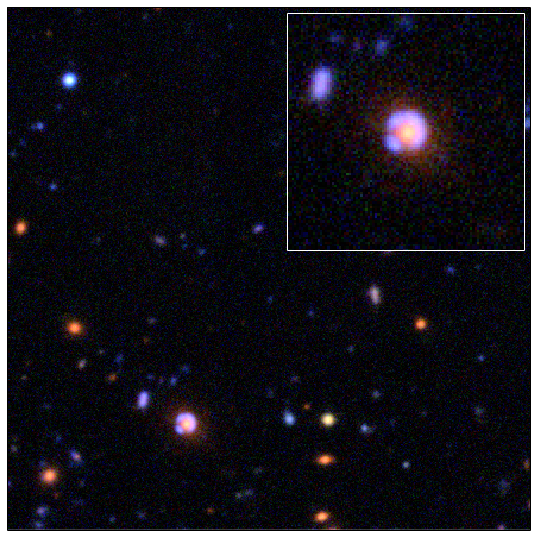
\epsfig{file=Figures/gallery/4.png,width=\linewidth,angle=0,clip=}
\end{minipage} \hfill
\begin{minipage}[b]{0.24\linewidth}
\centering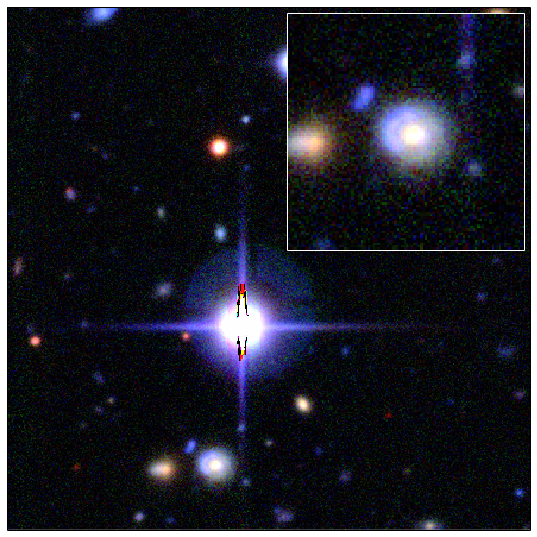
\epsfig{file=Figures/gallery/5.png,width=\linewidth,angle=0,clip=}
\end{minipage} \hfill
\begin{minipage}[b]{0.24\linewidth}
\centering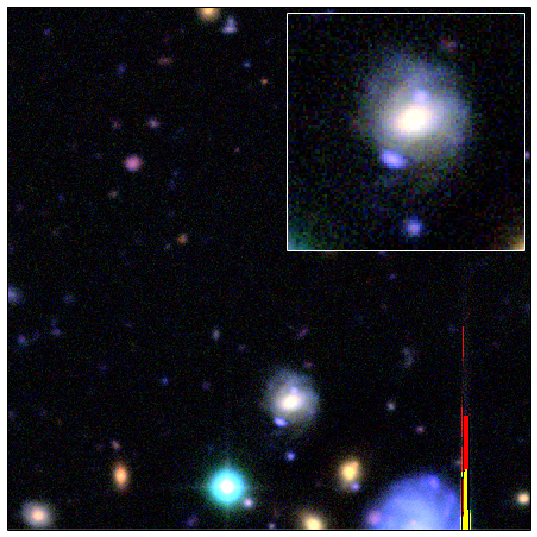
\epsfig{file=Figures/gallery/6.png,width=\linewidth,angle=0,clip=}
\end{minipage} \hfill
\begin{minipage}[b]{0.24\linewidth}
\centering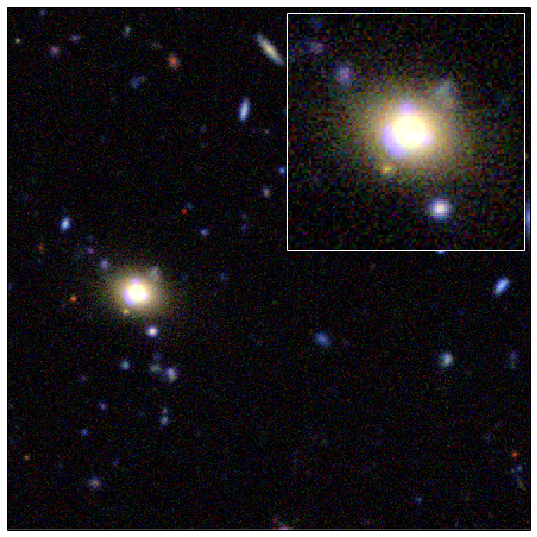
\epsfig{file=Figures/gallery/7.png,width=\linewidth,angle=0,clip=}
\end{minipage} \hfill
  \caption{Typical sims. Insets indicate the location of the lens in the
  image. These insets are fed into our training system.}
  \label{fig:sims}
\end{figure*}

\begin{figure*}[!ht]
\begin{minipage}[b]{0.24\linewidth}
\centering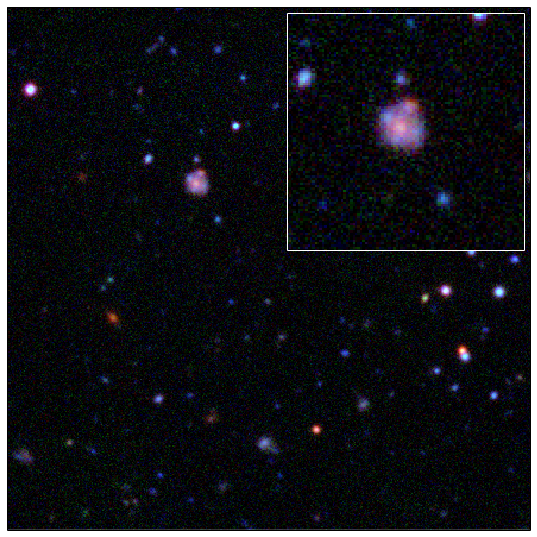
\epsfig{file=Figures/gallery/0.png,width=\linewidth,angle=0,clip=}
\end{minipage} \hfill
\begin{minipage}[b]{0.24\linewidth}
\centering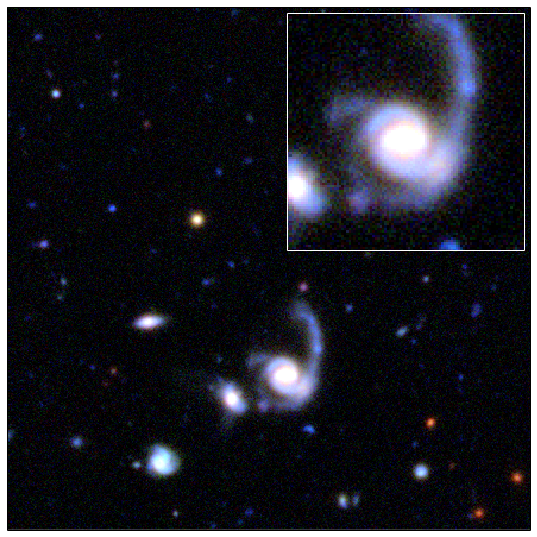
\epsfig{file=Figures/gallery/1.png,width=\linewidth,angle=0,clip=}
\end{minipage} \hfill
\begin{minipage}[b]{0.24\linewidth}
\centering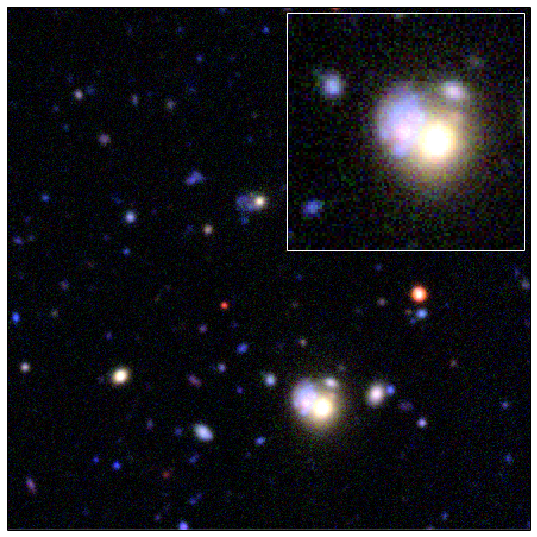
\epsfig{file=Figures/gallery/2.png,width=\linewidth,angle=0,clip=}
\end{minipage} \hfill
\begin{minipage}[b]{0.24\linewidth}
\centering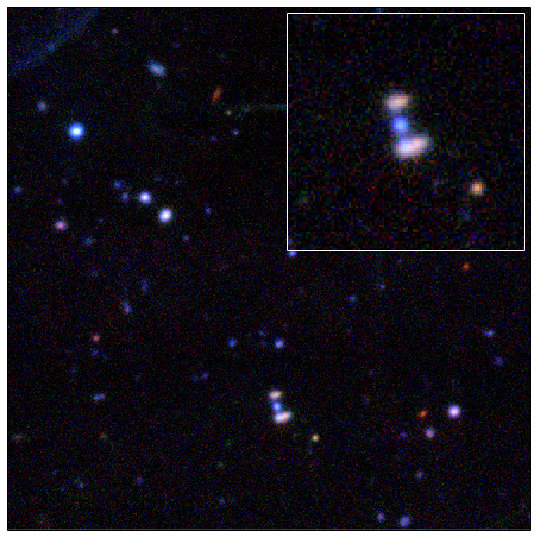
\epsfig{file=Figures/gallery/3.png,width=\linewidth,angle=0,clip=}
\end{minipage} \hfill
  \caption{Typical Space Warps duds. Insets indicate regions where volunteers
  typically clicked. These insets are then fed into our training system.}
  \label{fig:duds}
\end{figure*}

%-------------------------------------------------------------------------
\section{Problem Statement}

In this project we will use images collected by the Canada-France-Hawaii
Telescope Legacy Survey to analyze how Convolution Neural Networks can improve
automated detection of strong lens systems. We will also assess the performance
of citizen scientists by comparing our results to them. From other graduate
work (but not coursework), we have the locations and categories of around one
hundred and twenty known strong lenses, three thousand large fields verified to
contain no strong lenses, six thousand simulated strong lenses, and several
thousand classifications by citizen-scientists of other potential strong lens
systems.  These will form the core of our training and testing datasets; our
metric will be how well a CNN correctly identifies known and simulated lenses
and non-lens systems.

We would like to examine the following questions:
\begin{itemize}
\item{ Do we have enough data to reasonably train and test a CNN? Can we get
       around this by artificially inflating the data, e.g. by adding rotated
     images?}
\item{ How do citizen-scientists do compared with this automated system?}
\item{ Can we use the results of citizen-scientists to train the CNN?}
\item{ How well does using features extracted from a convolution neural network
       trained on galaxy morphology perform when determining the presence of
     strong gravitational lenses?}
\end{itemize}


%-------------------------------------------------------------------------
\section{Technical Approach}

From approximately 12000 fields of $440\times440\times3$ fields, we have
constructed approximately 30000 cutouts sized $96\times96\times3$. These cutouts
are selected based on where citizen scientists clicked, on the theory that both
'correct' and 'incorrect' selections provide useful information about the
characteristics of gravitational lenses. In general, we have access to two
broad classes of images: 'training' and 'test' images. The 'training' images
include fields that were verified in advance to not contain any lenses as well
as simulated lensed galaxies, quasars, and clusters. Many of the simulated
objects are over-exaggerated and extremely obvious, but we also have access to
a second 'refinement stage' of the project, where much harder simulations were
given to users. The 'test' images are the fields that citizen scientists
viewed, assessing whether a lens was in the field or not. In these 'test'
images are 120 known strong gravitational lens systems, which are also included
in this set. (The project confirms roughly half of these known lenses for
reasonable definitions of completeness and purity.) For all the images we also
have an associated probability that the project would evaluate that system as
containing a lens.

It is clear that we do not have enough data. Luckily, we also know that our
lens objects must obey certain symmetry properties, so it is quite easy to
augment our data. For example, we know that strong lens systems should be
independent of rotations as well as small amounts of stretching and
translation, so our data can be augmented by applying those transformations to
our images.

We train a classifier on this data using two different methods. First,
we code our own convolutional net in python using \textsc{theano}. Second,
we apply transfer learning techniques to train on a convolutional net
galaxy morphology classifier, which has graciously been made available to us by
Ryan Keisler and which achieved 7th place in the 2014 Galaxy Zoo Kaggle
competition.  This classifier runs $96\times96$ images through 3 convolutional
layers and 2 fully-connected layers and predicts a galaxy to have one of 37
enumerated morphologies. (See Figure~\ref{fig:ryan_architecture}.) We
train classifiers on top of the first fully-connected layer, which has 500
neurons.

%-------------------------------------------------------------------------
\subsection{The \textsc{Space Warps} Catalog}

\textsc{Space Warps} is a web-based service that enables the discovery of
strong gravitational lenses in wide-field imaging surveys by large numbers of
people. Carefully produced color composite images are displayed to volunteers
via a classification interface which records their estimates of the positions
of candidate lensed features. Simulated lenses, and expert-classified
non-lenses, are inserted into the image stream at random intervals; this
training set is used to give the volunteers feedback on their performance, and
to estimate a dynamically-updated probability for any given image to contain a
lens. Low probability systems are retired from the site periodically,
concentrating the sample towards a set of candidates; this ``stage 1'' set is
then re-classified by the volunteers in a second refinement stage. This ``stage
2'' has a different set of training images, ones that are generally considered
`harder'. Most stage 1 simulated lenses are very obvious\footnote{Very bright
and blue quasars multiply-imaged around a small red galaxy, very bright,
separated, and full \href{http://en.wikipedia.org/wiki/Einstein_ring}{Einstein
rings.}}, while simulated lenses in stage 2 are often much more subtle.
\footnote{Dim multiply-imaged quasars of varying magnitude, dim and incomplete
Einstein rings located close to a galaxy.} Figures~\ref{fig:duds} and
\ref{fig:sims}\xspace show example stage 2 fields with cutouts inlaid. Notice
that while the first three images in Figure~\ref{fig:sims} are very clearly
strong gravitational lenses \footnote{For the neophyte: the first is a broken
  blue arc around a central red galaxy; the second is a blue arc around a
  central yellow galaxy; the third is a multiply-imaged blue quasar (images
appear above and below the central galaxy), the fourth is a broken dim arc
located behind a very bright foreground galaxy.}, the fourth is very difficult
to find.  Unfortunately, we would very much like to find these, because there
are many such systems and they contain important information about the mass
structures at the centers of galaxies.\footnote{The trade off is this: the rate
  of alignment between foreground and background objects decreases as one
  decreases the area around a foreground object, but the strength of strong
  gravitational distortions -- and the signal we can pull out from identifying
  such systems -- increases as one gets closer to the center of the foreground
  object. A yet further complication to this is that background objects are
  naturally fainter than foreground objects, \textit{and} the foreground
  objects with the highest gravitational potential (and hence the largest
distortions of background images) tend to also be the brightest objects. Both
these complications render the task even more difficult.}
Figure~\ref{fig:duds} highlights the difficulties of this task. Each `dud' has
features that conceivably look like strong gravitational lensing, but are in
actuality some other confounding effect: color gradients from variations in the
Point Spread Function between the different color bands, dust surrounding a
galaxy, galaxies that are actually in the same cluster, and chance alignments
of background galaxies and foreground stars.

The fields users observe are $440\times440$ size images, containing multiple
potential locations for strong gravitational lenses, although it is unlikely
that a field contains more than one strong gravitational lens. In order to
generate $96\times96$ images of lenses and non-lenses, we use the recorded
estimates of the positions of candidate lensed feature. More specifically, we
apply the \textsc{DBSCAN} clustering algorithm, which agglomeratively grows
clusters such that that are within a minimum distance and contain a minimum
number of samples. \textsc{DBSCAN} is a convenient choice of a clustering
algorithm because it has a well-defined way of rejecting outliers, which we
generically interpret as genuine ``mis-clicks'' on the part of users. We are
very generous in the definition of a cluster and only require two members within
100 pixels of each other to form a cluster. 

The fear of noisy clusters is this: the real task of our techniques is to
distinguish strong gravitational lens systems from other configurations of
galaxies (for example, random alignments of galaxies). Noisy clicks end up
creating random cutouts of the field, slightly changing the task of our
classifier to distinguishing strong gravitational lens systems from random
cutouts from the field of a galaxy survey.  Inclusion of noise however ended up
not being an issue for stage 2: non-lenses, where the correct action on the
part of the user is to leave no marker, have a median of 28 markers in stage 2,
while simulated lenses (where the correct answer is to click at a specific
location) have a median of 180 markers. In stage 1, the simulated lenses have a
median of 80 markers, while the duds have a median of 3 markers (and a mean of
9.6). It may be the case that noise is injected in the stage 1 non-lens sample.

Overall, our base dataset has 24,177 images from stage 1, of which 5159 are of
simulated lenses, and 1876 images from stage 2, of which 151 are simulated
lenses. We also have 9030 classifications that stage 2 users made of images in
the CFHTLS survey where it is unknown whether they contain a lens or not. From
these classifications, a list of approximately 40 candidate strong
gravitational lensing objects have been found which will soon receive
spectroscopic follow-up to confirm whether they are strong gravitational
lensing systems or not.\footnote{Spectroscopy can yield precise redshifts of
  different objects in a field. This way, if different parts of a strong
  gravitational lens arc are at the same redshift, or if the multiply-imaged
quasars are, then one can confirm that we are really seeing such a system.} A
future project with this work would be to link the probabilities from the
\textsc{Space Warps} system with the probabilities obtained by a detection
algorithm.

%-------------------------------------------------------------------------
\section{Results}

% Not sure if we put anything here?

%-------------------------------------------------------------------------
\subsection{Convolution Neural Network}

% TODO: Insert figure for architecture

%-------------------------------------------------------------------------
\subsection{Transfer Learning}

% TODO: Touch up description
\begin{figure}%[!ht]
\centering
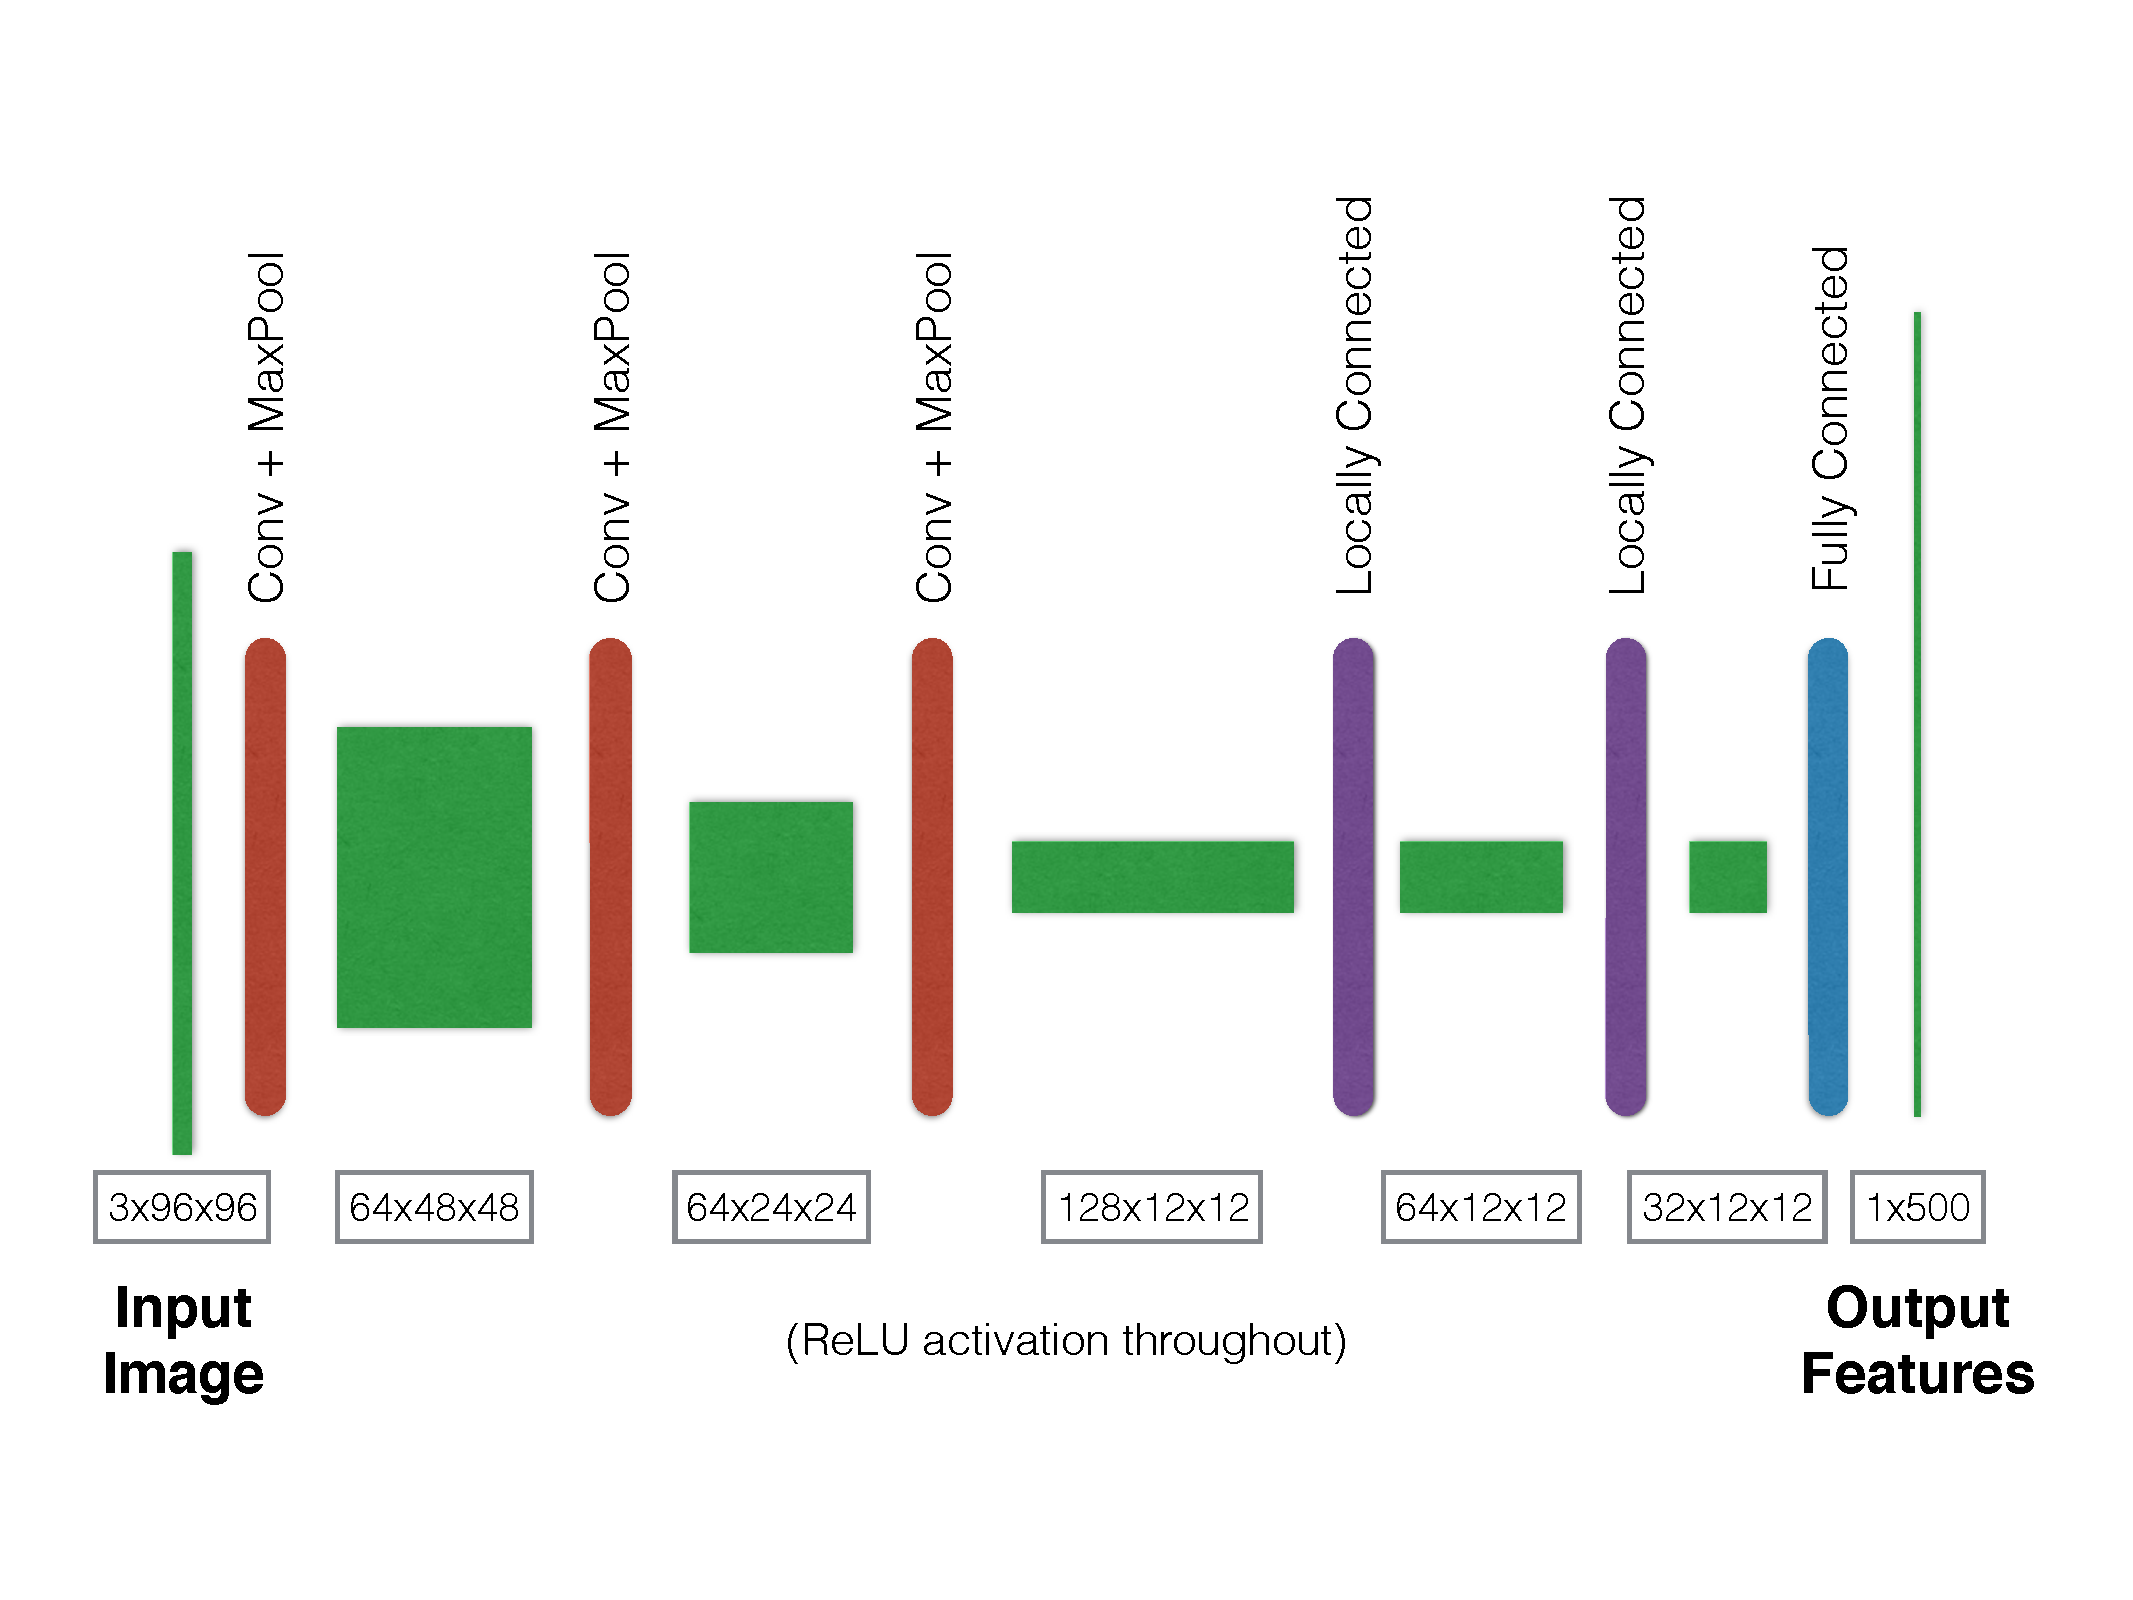
\epsfig{file=Figures/architecture.pdf,width=\linewidth,angle=0,clip=}
\caption{Architecture of the convolution
  neural network trained on the galaxy zoo morphologies. The feature vector we
use comes from the fully connected layer.}
\label{fig:ryan_architecture}
\end{figure}

\begin{figure*}%[!ht] 
\begin{minipage}[b]{0.48\linewidth}
\centering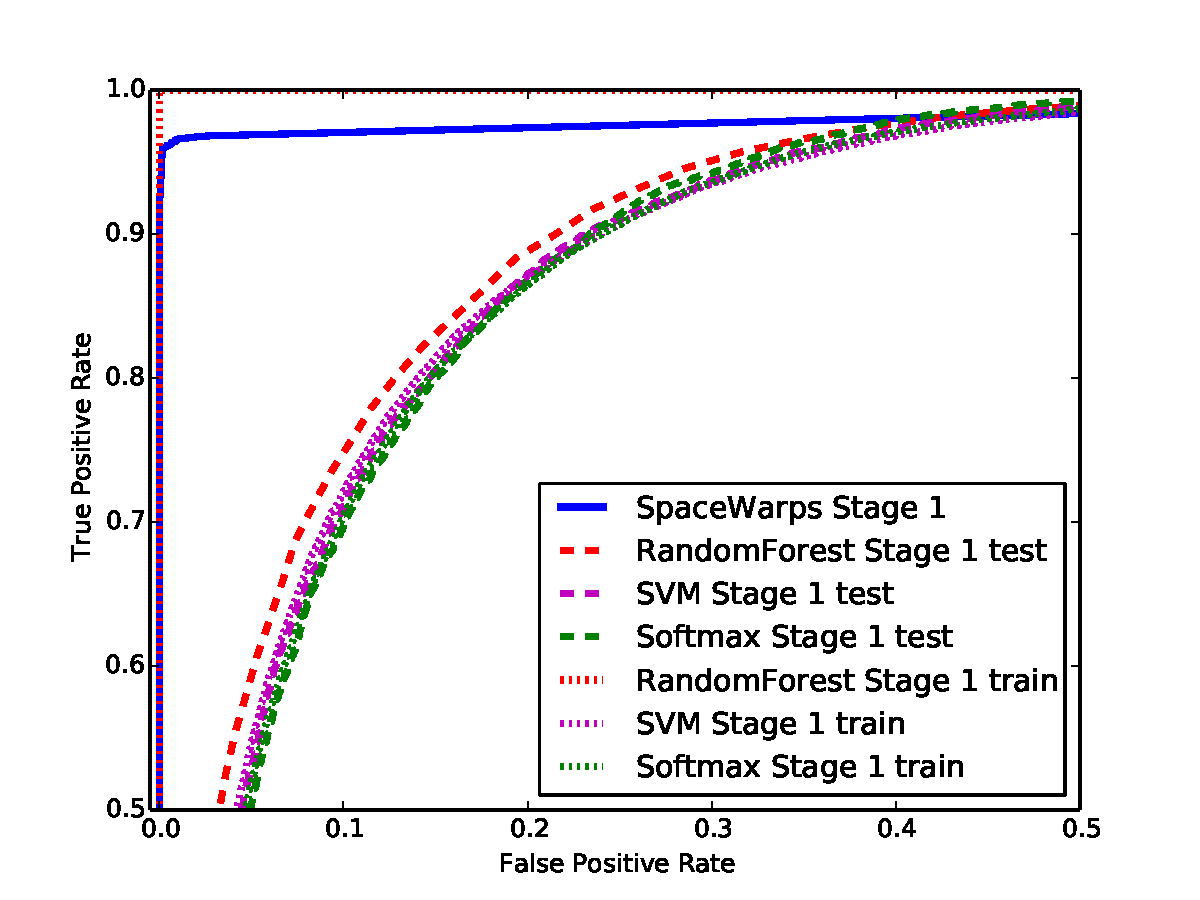
\epsfig{file=Figures/roc_curve_stage_1.pdf,width=\linewidth,angle=0,clip=}
\end{minipage} \hfill
\begin{minipage}[b]{0.48\linewidth}
\centering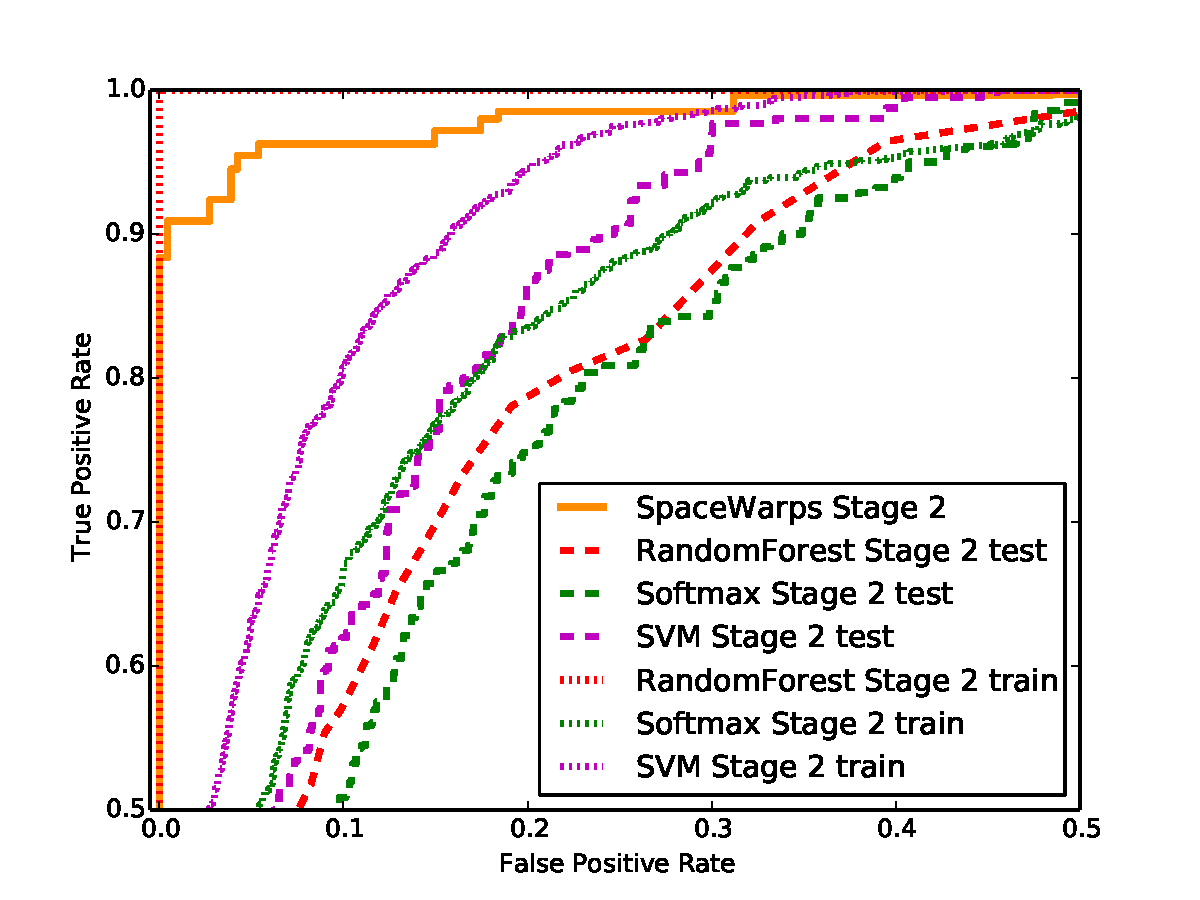
\epsfig{file=Figures/roc_curve_stage_2.pdf,width=\linewidth,angle=0,clip=}
\end{minipage} \hfill
  \caption{Receiver Operating Curves the \textsc{Space Warps} system and
    different linear classifiers trained on feature vectors extracted from a
    convolution neural network originally used to determine galaxy
  morphologies. We find that of the linear classifiers on the feature vectors,
support vector machine classifications perform best on the test dataset,
however all the feature vectors perform worse than the users themselves. Note
that the $x$-axis stops at a false positive rate of 0.5, and the $y$-axis
begins at a true positive rate of 0.5. Truly random guessing (which results in
a 1:1 relationship between the true positive rate and the false positive rate)
would not show up on this graph.}
\label{fig:roc_tl} 
\end{figure*}

Transfer Learning relies on the idea that convolution neural networks that
perform similar tasks pick up similar features, as well as the observation that
lower levels in neural networks tend to be quite generic in the features they
pick out. They provide an answer to the scenario when there are too few data to
effectively train a complex system like deep convolution neural networks: start
the training of your new system from the results of training a similar system.
For the scope of this project, we chose to examine the effects of transfer
learning from galaxy morphology to strong gravitational lens identification. In
both cases, an input image of a galaxy is fed into the network, and some
classification is read out. Additionally, both networks need to differentiate
shapes in the central regions of the galaxy image (for example to find bars in
spiral galaxies) from outer regions (spiral arms, arcs, multiply-lensed
systems). The Galaxy Zoo competition provides an ideal candidate for transfer
learning because of these facts, and also because the image quality is
comparable between the Sloan Digital Sky Survey (the telescope survey on which
the Galaxy Zoo images were based) and the CFHTLS survey. We have on hand a
convolution neural network trained to classify galaxy morphology provided by
Ryan Keisler \footnote{\url{rkeisler@stanford.edu}}. The architecture of that
network can be seen in Figure~\ref{fig:ryan_architecture}. We do the simplest
thing possible: we run the convolution neural network as a feature extractor,
and take images from the fully connected layer. Thus we transform a
$96\times96\times3$ image into a 500 feature vector. We then train these
feature vectors on various classifiers (Random Forest, Support Vector Machine,
Softmax) and evaluate results against a test set. We distinguish between stage
1 and stage 2 data because the simulated lenses changed between the two sets.
The code that produces the feature vectors also augments the data by
automatically producing feature vectors of flips and rotations of the input
images. This allows us to increase the size of our input dataset nearly
20-fold.

We train these datasets on three classifiers: Random Forests (which are an
ensemble of decision trees trained on the data), Softmax and linear Support
Vector Machines. We use stochastic gradient descent for the latter two
classifiers. We create a test dataset by randomly extracting 20 percent of the
dataset and setting it aside. We also ensure that any data augmentation stays
in the training or test sets. Our goal with all the above systems is not to
find the maximal accuracy, but to find some reasonable trade-off between the
true positive rate and the false positive rate: we want to find as many lenses
as we can, but we also know that confirmation of these lenses by spectroscopic
follow-up is an expensive endeavor such that we want to minimize the number of
non-lenses that make it into our candidate list. Because of this, any potential
candidate list we would make from any of our classifiers has a relatively hard
threshold at a false positive rate of 0.2.

The resultant Receiver Operating Curves can be observed in
Figure~\ref{fig:roc_tl}. In general we find that support vector machines
perform the best as a classifier on the feature vectors, but that the feature
vectors perform more poorly than the \textsc{Space Warps} users. We must caveat
though that \textsc{Space Warps} does not create a validation dataset against
which to test the performance of the system. Even if we don't perform quite as
well as the citizen scientists, we consider this a
promising baseline for future performance by transfer learning: we have not
even begun to consider potential performance gains by retraining the
convolution neural network on the \textsc{Space Warps} data.

%-------------------------------------------------------------------------
\section{Discussion}

% Do we need this section?

%-------------------------------------------------------------------------
\section{Conclusions}

% Discuss how well things went. Or didn't go.
The need for new automated detection algorithms for finding strong
gravitational lenses will only become more pressing in the next decade, as it
becomes infeasible for scientists to scan images by eye for such systems. Using
the \textsc{Space Warps} dataset, we have examined how convolution neural
networks trained both on this particular dataset and on other datasets can
perform at the detection task.
% TODO: brief blurb about our CNN
We find that features extracted from a convolution neural network trained on
the classification of galaxy morphology (with a linear support vector
classifier on top for converting the feature vector to a binary ``lens'' and
``not-lens'') performs admirably but markedly worse than the citizen scientists
trained on the dataset. Further work examining improvements by retraining the
whole neural network could lead to a generic classification machine that takes
images from \textit{any} galaxy survey and states whether the image contains a
strong lens or not. Additionally there is much potential in both direct
convolution neural networks and transfer learning from other networks in
linking the classification outputs of the networks with the probability
estimates of the \textsc{Space Warps} system, which also examined several
thousands more ``unknown'' systems and could lead to more gravitational lenses
being identified.

%-------------------------------------------------------------------------
\section{Acknowledgements}
We received access to the dataset through Phil Marshall
\footnote{\url{pjm@slac.stanford.edu}}, who also graciously explained to us how
\textsc{Space Warps}
currently works. The convolutional neural network upon which the transfer
learning is based was kindly provided to us by Ryan Keisler
\footnote{\url{rkeisler@stanford.edu}}.
All errors in interpretation or otherwise are entirely our own.

%-------------------------------------------------------------------------
% References

% TODO: copy relevant bib stuff over so I don't have a 4 mb bib
{\small
\bibliographystyle{ieee}
\bibliography{coursebib}
}

\end{document}
